\section{Задание 4. Системы ДУ. Устойчивость.}

\textbf{Условие.}

Дана система ДУ:

\[\begin{cases}
      \frac{dx}{dt} = -2x + 5y, \\ \frac{dy}{dt} = 2x + y
\end{cases}\]

\begin{enumerate}
    \item Найдите общее решение системы.
    \item Изобразите на фазовой плоскости семейство интегральных кривых $y = y(x)$.
    \item Исследуйте решение системы на устойчивость при $t \to +\infty$.
    \item Определите характер особой точки.
\end{enumerate}

\vspace{10mm}
\textbf{Решение.}

\begin{enumerate}
    \item Решение ДУ

    Решим через метод Эйлера (через характеристическое уравнение).

    В общем наше решение будет выглядеть как система функций вида:

    \begin{equation*}
        \begin{cases}
            x(t) = \omega_1 C_1 e^{\lambda_1t} + \omega_2 C_2 e^{\lambda_1t}
            \\
            y(t) = \mu_1 C_1 e^{\lambda_2t} + \mu_2 C_2 e^{\lambda_2t}
        \end{cases}
    \end{equation*}


    $\displaystyle \begin{vmatrix}
                       -2 & 5 \\
                       2  & 1 \\
    \end{vmatrix} = $
    $\displaystyle \begin{vmatrix}
                       -2 - \lambda & 5           \\
                       2            & 1 - \lambda \\
    \end{vmatrix} $

    $(-2-\lambda)(1-\lambda) - 2 \cdot 5 = 0$
    $\Rightarrow \lambda^2 + \lambda - 12 = 0$
    $\Rightarrow \lambda_{1,2} = -4, 3$

    \begin{multicols}{2}
        \begin{subtasks}
            \item $\lambda_1 = -4$
            $\displaystyle \begin{vmatrix}
                               2 & 5 \\
                               2 & 5 \\
            \end{vmatrix} \Rightarrow \omega_1 = -\frac{5}{2} \mu_1 $ \\ (возьмем $\mu_2 = 1$, тогда $\omega_1 = -\frac{5}{2}$).
            \item $\lambda_2 = 3$
            $\displaystyle \begin{vmatrix}
                               -5 & 5  \\
                               2  & -2 \\
            \end{vmatrix} \Rightarrow \omega_2 = \mu_2 $ \\ (возьмем любое число, к примеру: 1).
        \end{subtasks}
    \end{multicols}

    Тогда наша система выглядит так:

    \begin{equation*}
        \begin{cases}
            x(t) = -\frac{5}{2} C_1 e^{-4t} + C_2 e^{3t}
            \\
            y(t) = C_1 e^{-4t} + C_2 e^{3t}
        \end{cases}
    \end{equation*}


    \item Фазовая плоскость

    Т.к. собственные числа характеристического уравнения действительные и разных знаков то фазовая плоскость будет состоять
    как бы из гипербол. Поэтому нам нужно найти векторы асимптот. Каждый такой вектор $x_i$ можно найти через уравнение

    $\displaystyle \begin{vmatrix}
                       -2 - \lambda_i & 5             \\
                       2              & 1 - \lambda_i \\
    \end{vmatrix} \cdot x_i =
    \begin{pmatrix}
        0 \\
        0 \\
    \end{pmatrix}
    $

    Таким образом: $
    x_1 =
    \begin{pmatrix}
        5  \\
        -2 \\
    \end{pmatrix} ,
    x_2 =
    \begin{pmatrix}
        -1 \\
        -1 \\
    \end{pmatrix}
    $

    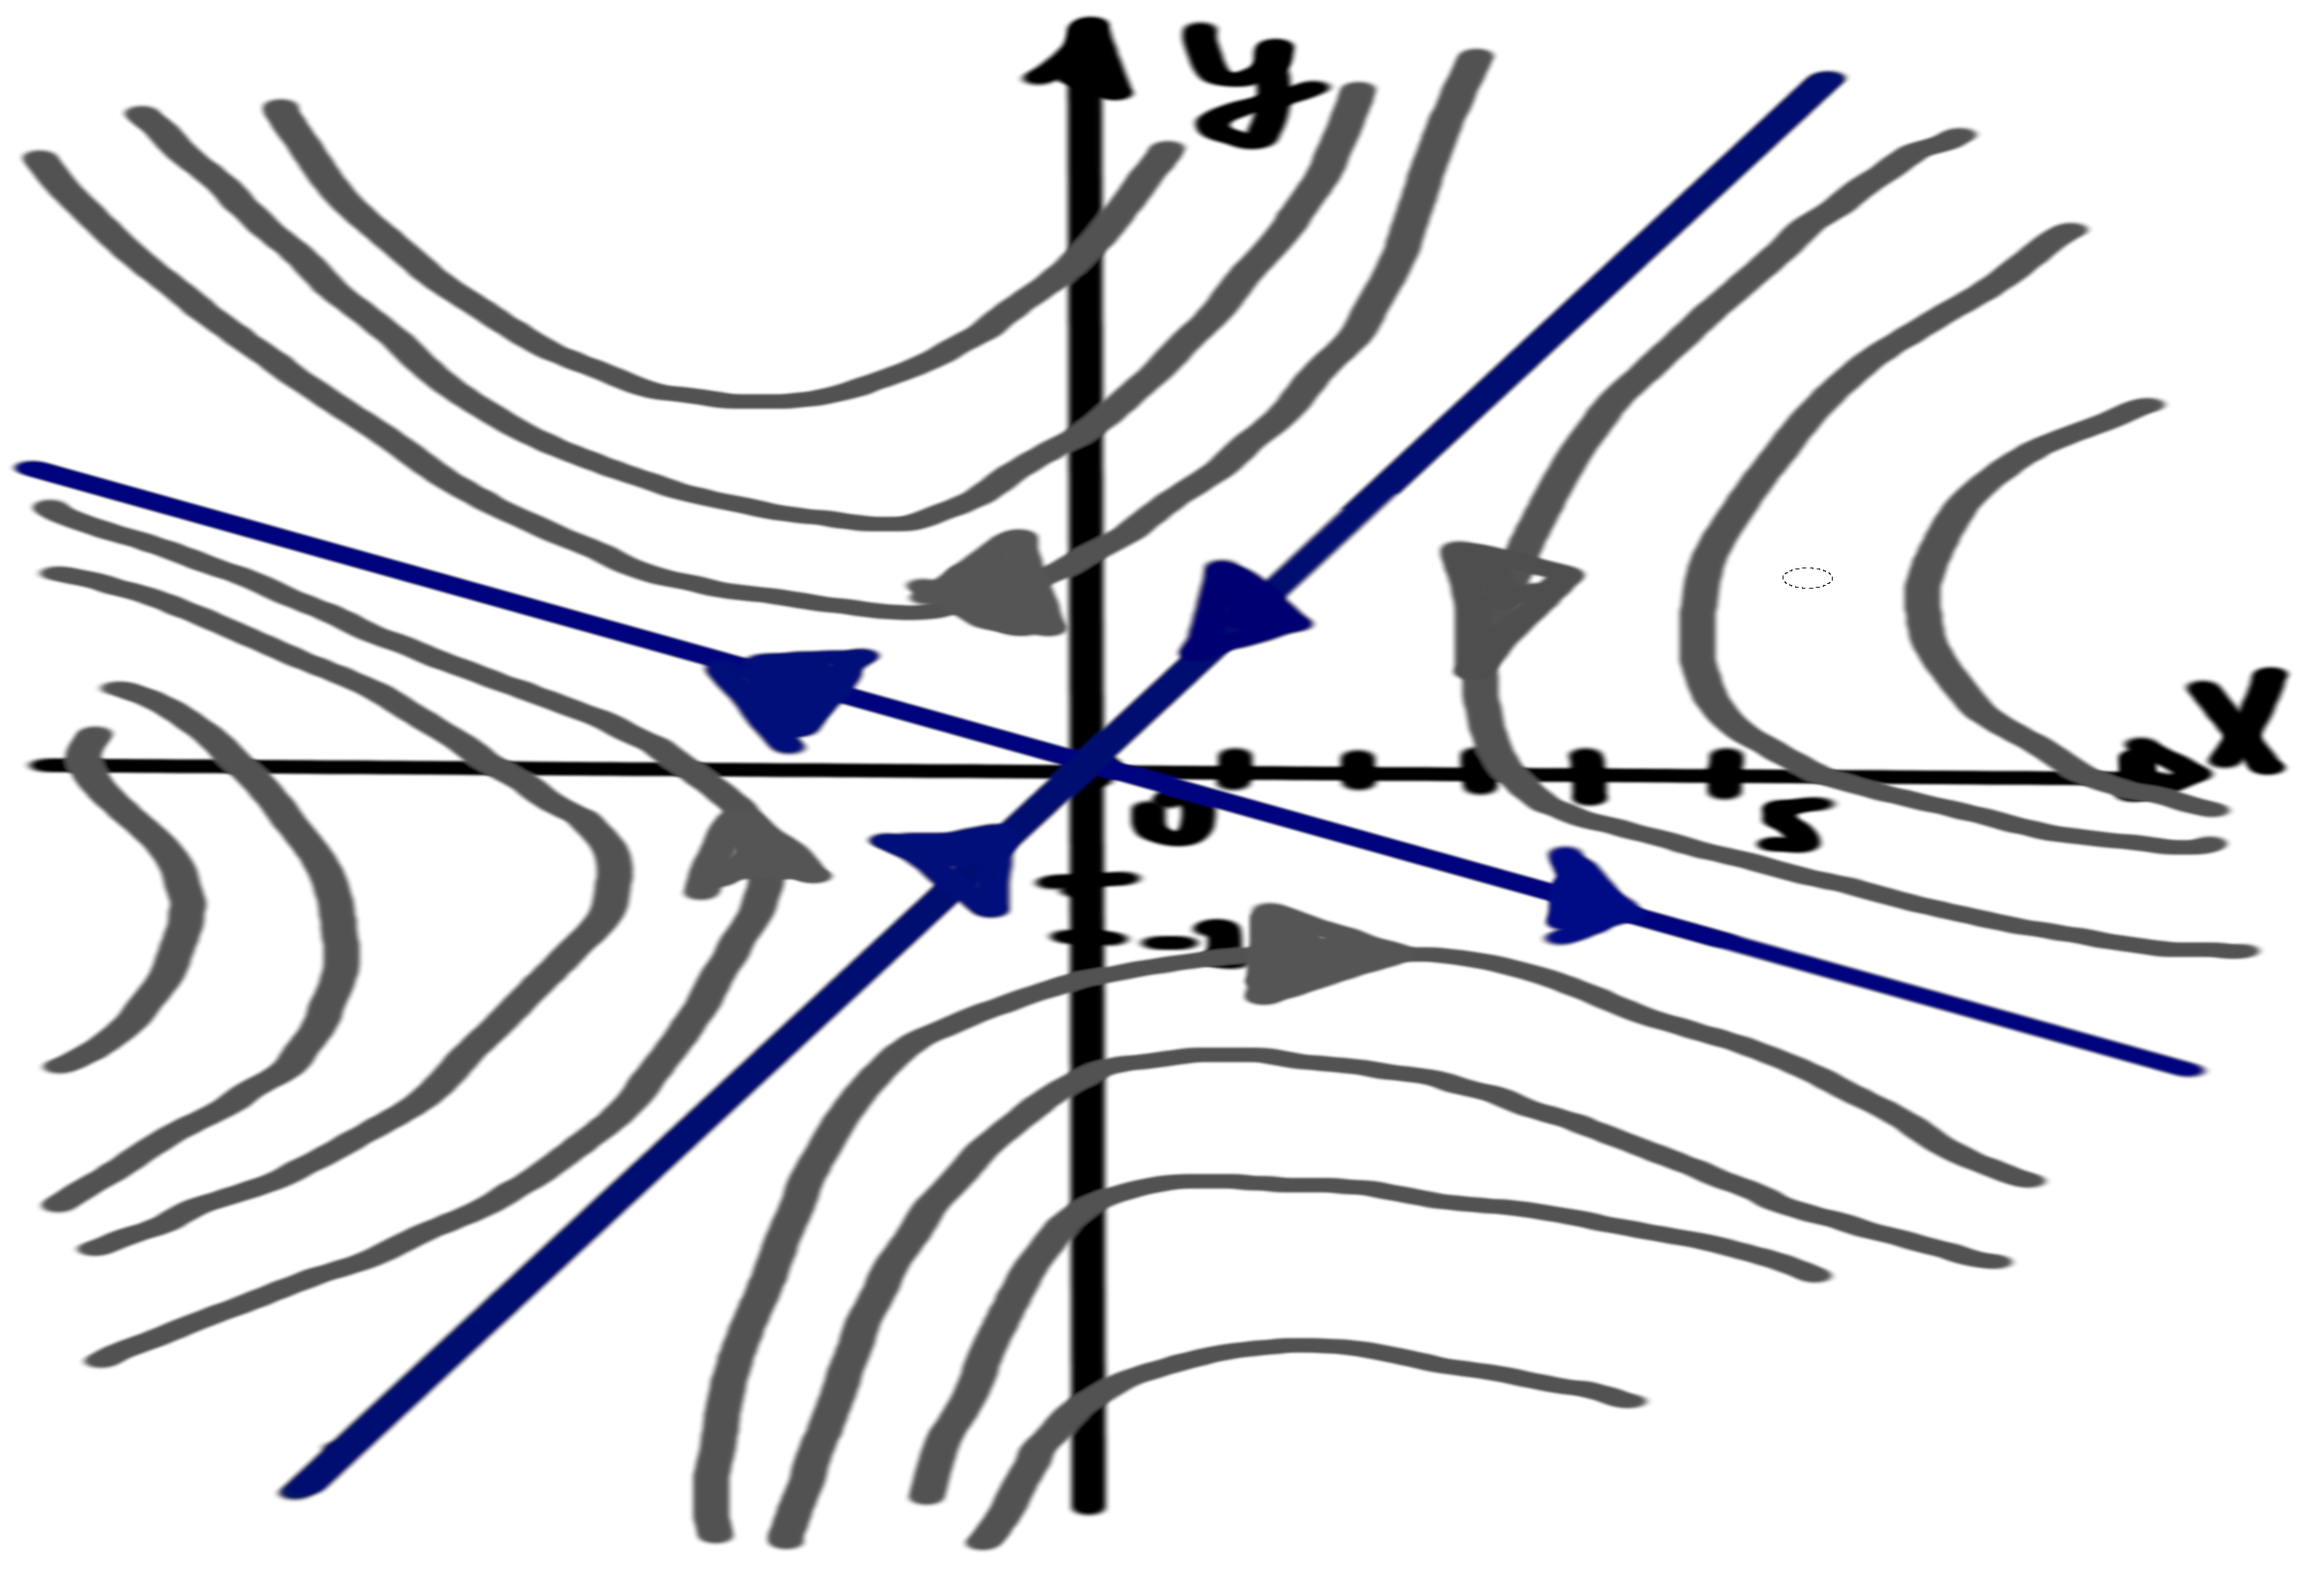
\includegraphics[scale=0.2]{images/4a1}

    \item Устойчивость: Т.к. корни характеристического уравнения действительные числа одного знака, то
    положение равновесия которое у нас получится - седло.
    \item Тип особой точки: (0, 0) - седло
\end{enumerate}

